\documentclass[12pt,a4paper]{report}
\usepackage[T2A]{fontenc}
\usepackage[utf8]{inputenc}
\usepackage[russian]{babel}
\usepackage{graphicx, setspace, amsmath, multirow}

\usepackage[
top = 1.25cm, 
bottom = 2.0cm]{geometry}

\begin{document}
\begin{titlepage}
	\centering
	% HEADER
	{
		\scshape
		Федеральное государственное автономное образовательное учреждение высшего образования
		\par
		\textbf{«Научно-образовательная корпорация ИТМО»}
		\par
		\vspace*{1cm}
		Факультет Программной Инженерии и Компьютерной Техники
		\par
	}
	% LOGO
	\vspace*{0.6cm}
	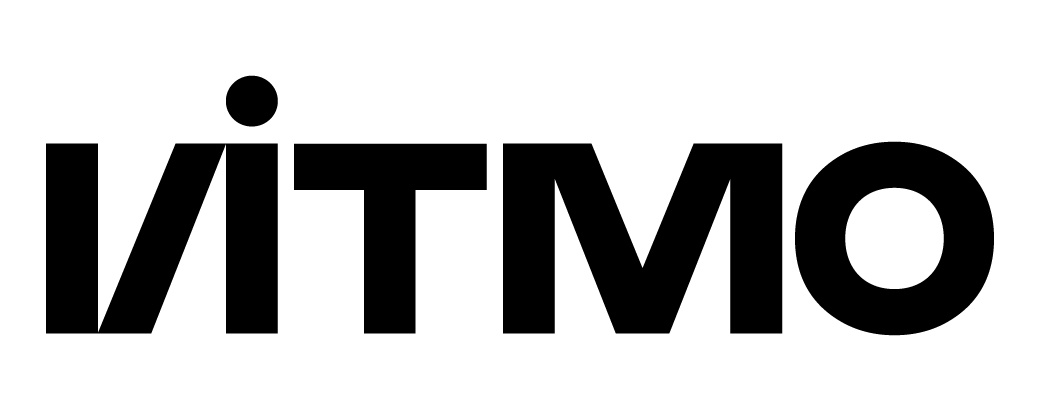
\includegraphics[width=\textwidth]{logo.png}
	% LAB INFO
	{
		\Large
		\textbf{Индивидуальное домашнее задание №2}
		\par
		\normalsize
		\vspace*{0.75cm}
		\textbf{Вариант 12}
		\par
	}
	\vfill
	% СREDITS
	\hfill\begin{minipage}{\dimexpr\textwidth-7.8cm}
		\textbf{Выполнил:}\par
		Степанов Арсений Алексеевич\par
		\vspace*{0.15cm}
		\textbf{Группа:}\par
		ТеорВер 2.4\par
		\vspace*{0.15cm}
		\textbf{Преподаватель:}\par
		Селина Елена Георгиевна\par
	\end{minipage}
	\vfill
	Санкт-Петербург, \the\year{}г.
\end{titlepage}
\section*{Задание №1}
\subsection*{Исходные данные}
\begin{tabular}{|c|c|c|c|c|c|c|c|c|c|}
	\hline
	32  & 105 & 48  & 80  & 144 & 128 & 64  & 112 & 18  & 81  \\
	\hline
	66  & 129 & 113 & 17  & 94  & 78  & 90  & 51  & 104 & 34  \\
	\hline
	110 & 149 & 36  & 103 & 82  & 53  & 93  & 130 & 68  & 150 \\
	\hline
	114 & 84  & 55  & 131 & 70  & 38  & 102 & 77  & 16  & 135 \\
	\hline
	41  & 19  & 142 & 61  & 85  & 159 & 115 & 57  & 72  & 101 \\
	\hline
	56  & 100 & 86  & 146 & 73  & 40  & 141 & 25  & 87  & 126 \\
	\hline
	151 & 71  & 94  & 15  & 125 & 76  & 54  & 99  & 39  & 140 \\
	\hline
	17  & 124 & 52  & 98  & 139 & 37  & 147 & 88  & 69  & 109 \\
	\hline
	35  & 158 & 67  & 30  & 93  & 123 & 50  & 138 & 21  & 97  \\
	\hline
	96  & 121 & 49  & 137 & 89  & 145 & 91  & 65  & 92  & 33  \\
	\hline
\end{tabular}
\subsection*{Вариационный ряд}
\begin{tabular}{|c|c|c|c|c|c|c|c|c|c|}
	\hline
	15  & 16  & 17  & 17  & 18  & 19  & 21  & 25  & 30  & 32  \\
	\hline
	33  & 34  & 35  & 36  & 37  & 38  & 39  & 40  & 41  & 48  \\
	\hline
	49  & 50  & 51  & 52  & 53  & 54  & 55  & 56  & 57  & 61  \\
	\hline
	64  & 65  & 66  & 67  & 68  & 69  & 70  & 71  & 72  & 73  \\
	\hline
	76  & 77  & 78  & 80  & 81  & 82  & 84  & 85  & 86  & 87  \\
	\hline
	88  & 89  & 90  & 91  & 92  & 93  & 93  & 94  & 94  & 96  \\
	\hline
	97  & 98  & 99  & 100 & 101 & 102 & 103 & 104 & 105 & 109 \\
	\hline
	110 & 112 & 113 & 114 & 115 & 121 & 123 & 124 & 125 & 126 \\
	\hline
	128 & 129 & 130 & 131 & 135 & 137 & 138 & 139 & 140 & 141 \\
	\hline
	142 & 144 & 145 & 146 & 147 & 149 & 150 & 151 & 158 & 159 \\
	\hline
\end{tabular}\\
\hfill\break
Размах выборки $R=x_{\max}-x_{\min}=159-15=144$ \\
Величина интервала находится по формуле: $h=\frac{144}{9}=16$ \\

\begin{tabular}{|c|c|c|c|}
	\hline
	Интервал $[x_i, x_{i+1})$ & $n_i$ & $w_i, w_i=\frac{n_i}{nh}$ & $f_i, f_i=\frac{n_i}{n}$ \\
	\hline
	15-31                     & 9     & 0.005625                  & 0.09                     \\
	\hline
	31-47                     & 10    & 0.00625                   & 0.19                     \\
	\hline
	47-63                     & 11    & 0.006875                  & 0.3                      \\
	\hline
	63-79                     & 13    & 0.008125                  & 0.43                     \\
	\hline
	79-95                     & 16    & 0.01                      & 0.59                     \\
	\hline
	95-111                    & 12    & 0.0075                    & 0.71                     \\
	\hline
	111-127                   & 9     & 0.005625                  & 0.8                      \\
	\hline
	127-143                   & 11    & 0.006875                  & 0.91                     \\
	\hline
	143-159                   & 9     & 0.005625                  & 1                        \\
	\hline
\end{tabular}

\subsection*{Полигон частот}
\begin{center}
	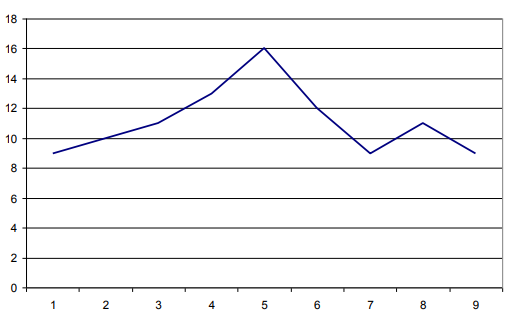
\includegraphics[width=10cm]{polygon.png}
\end{center}
\subsection*{Гистограмма}
\begin{center}
	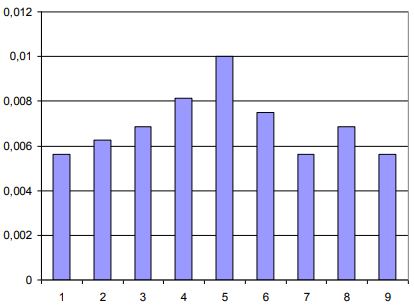
\includegraphics[width=10cm]{histo.png}
\end{center}
\subsection*{Эмпирическая функция распределения}
\begin{center}
	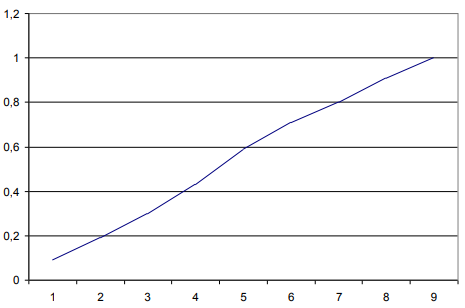
\includegraphics[width=10cm]{function.png}
\end{center}
\subsection*{Числовые характеристики выборки}
$$\overline{x}=\sum_{i=1}^{9}\frac{x_i'n_i}{n}=86.68\qquad D=\sum_{i=1}^{9}\frac{(x_i-\overline{x})^2n_i}{n}=1489.82$$
Приняв в качестве нулевой гипотезу $H_0$: генеральная совокупность, из которой извлечена выборка, имеет нормальное распределение, проверить ее, пользуясь критерием Пирсона при уровне значимости $\alpha$ = 0.025\\
\hfill\break
Перейдём к новой случайной величине $Z=\frac{X-\overline{x}}{\sqrt{D}}$ и вычислим концы интервалов $z_i=\frac{x_i-\overline{x}}{\sqrt{D}}$\\
\hfill\break
$n_i'=n\cdot P_i$, $P_i=\Phi(z_{i + 1})-\Phi(z_i)$\\
\hfill\break
\begin{tabular}{|c|c|c|c|c|}
	\hline
	$Z_i$    & $Z_i + 1$ & $n_i'$   & $n_i$ & $\frac{(n_i-n_i')^2}{n_i'}$ \\
	\hline
	0.0      & -1,44256  & 7.45728  & 9     & 0.319149                    \\
	\hline
	-1.44256 & -1.02803  & 7.739544 & 10    & 0.660202                    \\
	\hline
	-1.02803 & -0.6135   & 11.78044 & 11    & 0.051703                    \\
	\hline
	-0.6135  & -0.19897  & 15.13692 & 13    & 0.301675                    \\
	\hline
	-0.19897 & 0.215554  & 16.41906 & 16    & 0.010696                    \\
	\hline
	0.215554 & 0.630082  & 15.03471 & 12    & 0.612546                    \\
	\hline
	0.630082 & 1.04461   & 11.62188 & 9     & 0.591491                    \\
	\hline
	1.04461  & 1.459137  & 7.583805 & 11    & 1.538856                    \\
	\hline
	1.459137 & 0.0       & 7.226369 & 9     & 0.435318                    \\
	\hline
\end{tabular}\\
\hfill\break
$$\chi_{\text{набл}}=\sum_{i=1}^9\frac{(n_i-n_i')^2}{n_i'}=4.5216$$
По таблице квантилей распределения $\chi^2$ по заданному уровню значимости $\alpha$ и числу степеней свободы $k=9-3=6$, можно найти критическое значение $\chi^2_\text{крит}=14.45$, а так как $\chi^2_\text{набл}<\chi^2_\text{крит}$, то распределение можно считать нормальным на уровне значимости $\alpha=0.25$
\subsection*{Доверительные интервалы выборки}
Находим доверительные интервалы для математического ожидания и
среднеквадратического отклонения с доверительной вероятностью $\gamma=0.9$\\
\hfill\break
Доверительный интервал находится по формуле:
$$(\overline{x}-\frac{t_\gamma S}{\sqrt{n}}; \overline{x}+\frac{t_\gamma S}{\sqrt{n}})\qquad S=\sqrt{\frac{n}{n-1}D}$$ \\
$$t_\gamma=1.66\qquad S=38.79\Rightarrow MX\in(80.24; 93.12)$$
Доверительный интервал для среднеквадратического отклонения находится по формуле:
$$(\frac{S\sqrt{n-1}}{\chi_2}; \frac{S\sqrt{n-1}}{\chi_1})$$\\
\hfill\break
$\chi_1$ и $\chi_2$ - квантили распределения $\chi^2$ уровня $\frac{1-\gamma}{2}=0.05$ и $1-\frac{1-\gamma}{2}=0.95$ с 99 степенями свободы\\
\hfill\break
$\chi_1=8.77$, $\chi_2=11.1$, тогда $\sigma \in (\frac{\sqrt{99}\cdot38.79}{11.1}; \frac{\sqrt{99}\cdot38.79}{8.77})$
$$\sigma\in(34.77;44.01)$$
\section*{Задание №2}
\subsection*{Исходные данные}
\begin{tabular}{|c|cccccccc|c|}
	\hline
	\multirow{2}{*}{$X$} & \multicolumn{8}{c|}{$Y$} & \multirow{2}{*}{$m_x$}                                                                                                                                                      \\ \cline{2-9}
	                     & \multicolumn{1}{c|}{110} & \multicolumn{1}{c|}{130} & \multicolumn{1}{c|}{150} & \multicolumn{1}{c|}{170} & \multicolumn{1}{c|}{190} & \multicolumn{1}{c|}{210} & \multicolumn{1}{c|}{230} & 250 &     \\ \hline
	10                   & \multicolumn{1}{c|}{1}   & \multicolumn{1}{c|}{3}   & \multicolumn{1}{c|}{4}   & \multicolumn{1}{c|}{-}   & \multicolumn{1}{c|}{-}   & \multicolumn{1}{c|}{-}   & \multicolumn{1}{c|}{-}   & -   & 8   \\ \hline
	13                   & \multicolumn{1}{c|}{-}   & \multicolumn{1}{c|}{5}   & \multicolumn{1}{c|}{6}   & \multicolumn{1}{c|}{5}   & \multicolumn{1}{c|}{-}   & \multicolumn{1}{c|}{-}   & \multicolumn{1}{c|}{-}   & -   & 16  \\ \hline
	16                   & \multicolumn{1}{c|}{-}   & \multicolumn{1}{c|}{-}   & \multicolumn{1}{c|}{4}   & \multicolumn{1}{c|}{8}   & \multicolumn{1}{c|}{6}   & \multicolumn{1}{c|}{-}   & \multicolumn{1}{c|}{-}   & -   & 18  \\ \hline
	19                   & \multicolumn{1}{c|}{-}   & \multicolumn{1}{c|}{-}   & \multicolumn{1}{c|}{6}   & \multicolumn{1}{c|}{15}  & \multicolumn{1}{c|}{9}   & \multicolumn{1}{c|}{-}   & \multicolumn{1}{c|}{-}   & -   & 30  \\ \hline
	22                   & \multicolumn{1}{c|}{-}   & \multicolumn{1}{c|}{-}   & \multicolumn{1}{c|}{-}   & \multicolumn{1}{c|}{-}   & \multicolumn{1}{c|}{5}   & \multicolumn{1}{c|}{6}   & \multicolumn{1}{c|}{7}   & -   & 18  \\ \hline
	25                   & \multicolumn{1}{c|}{-}   & \multicolumn{1}{c|}{-}   & \multicolumn{1}{c|}{-}   & \multicolumn{1}{c|}{-}   & \multicolumn{1}{c|}{-}   & \multicolumn{1}{c|}{1}   & \multicolumn{1}{c|}{7}   & 2   & 10  \\ \hline
	$m_y$                & \multicolumn{1}{c|}{1}   & \multicolumn{1}{c|}{8}   & \multicolumn{1}{c|}{20}  & \multicolumn{1}{c|}{28}  & \multicolumn{1}{c|}{20}  & \multicolumn{1}{c|}{7}   & \multicolumn{1}{c|}{14}  & 2   & 100 \\ \hline
\end{tabular}
\subsection*{Решение}
Найдём выборочные средние $x$ и $y$:
$$x=\frac{1}{n}\sum_{i=1}^{6}\sum_{j=1}^{8}m_{ij}x_i=\frac{1792}{100}=17.92\qquad y=\frac{1}{n}\sum_{i=1}^{6}\sum_{j=1}^{8}m_{ij}y_i=\frac{17900}{100}=179$$
Найдём выборочные дисперсии:
$$S_x^2=\frac{1}{n-1}(\sum_{i=1}^{6}\sum_{j=1}^{8}m_{ij}x_i^2-\frac{1}{n}(\sum_{i=1}^{6}\sum_{j=1}^{8}m_{ij}x_i)^2)=\frac{1}{99}(33904-\frac{1}{100}1792^2)=18.0945$$
$$S_y^2=\frac{1}{n-1}(\sum_{i=1}^{6}\sum_{j=1}^{8}m_{ij}y_i^2-\frac{1}{n}(\sum_{i=1}^{6}\sum_{j=1}^{8}m_{ij}y_i)^2)=\frac{1}{99}(3302800-\frac{1}{100}17900^2)=996.97$$
Найдём корреляционный момент:
$$S_{xy}=\frac{1}{n-1}(\sum_{i=1}^{6}\sum_{j=1}^{8}m_{ij}x_iy_j-\frac{1}{n}(\sum_{i=1}^{6}\sum_{j=1}^{8}m_{ij}x_i)(\sum_{i=1}^{6}\sum_{j=1}^{8}m_{ij}y_i))$$
$$S_{xy}=\frac{1}{99}(331880-\frac{1}{100}(1792\cdot 17900))=112.242$$
Найдём уравнение эмпирической линии регрессии:
$$S_x=\sqrt{18.0945}=4.2538\qquad S_y=\sqrt{996.97}=31.5748\qquad r_{xy}=\frac{S_{xy}}{S_x\cdot S_y}=0.8357$$
$$y=y_0+r_{xy}\frac{S_y}{S_x}(x-x_0)=179+0.8357\cdot\frac{31.5748}{4.2538}\cdot(x-17.92)=6.20311x+67.8403$$
\subsection*{Линия регрессии и случайные точки}
\begin{center}
	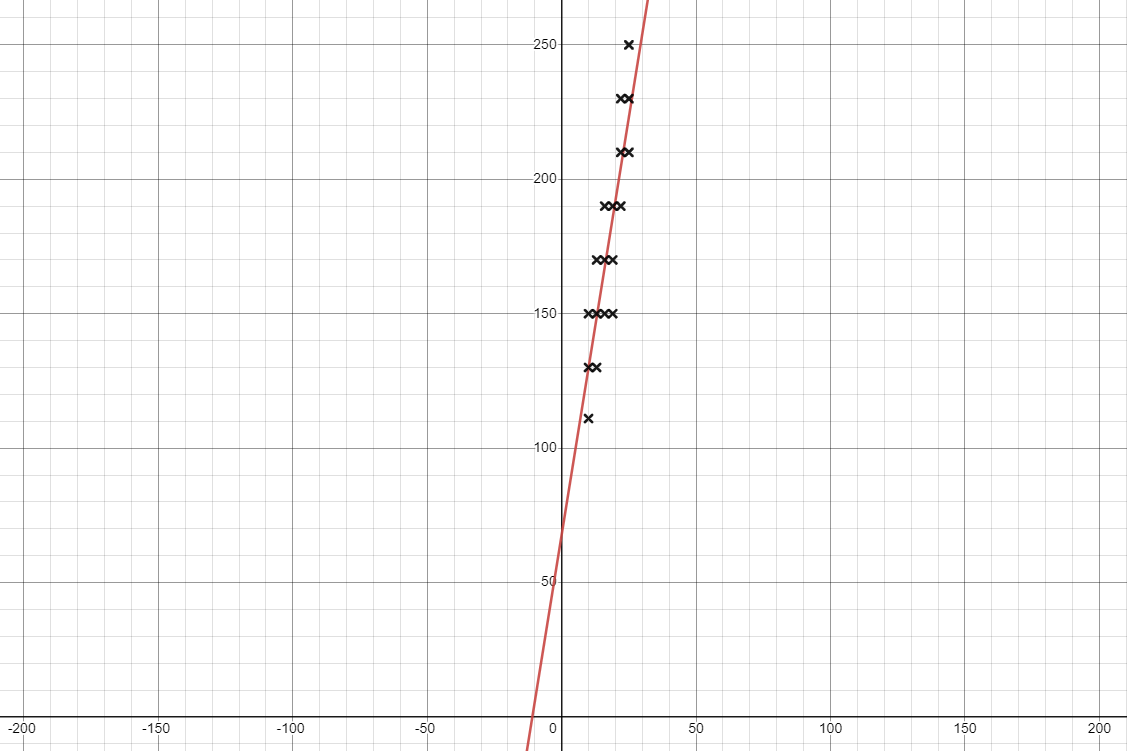
\includegraphics[width=\textwidth]{regression.png}
\end{center}
\end{document}